\section{Menusystem}\label{sec:menu}
For at kunne ændre på equalizerens parametre og indstillinger, skal der være en form for menusystem. Dette menusystem skal opbygges på en måde, så det ikke forstyrrer mikroprocessorens andre igangværende processer (såsom håndtering af lydsignalet som er den primære funktion). Derfor opsættes en buffer som kan modtage data når det bliver tilgængeligt, og når der er tid til at håndtere dette. Visning af menu på displayet og håndtering af de diverse inputs, skal foregå meget enkelt, da der i alt kun er 1024 clock cycles tilbage efter håndtering af lydsignalet. \\

\begin{figure}[h]
	\centering
	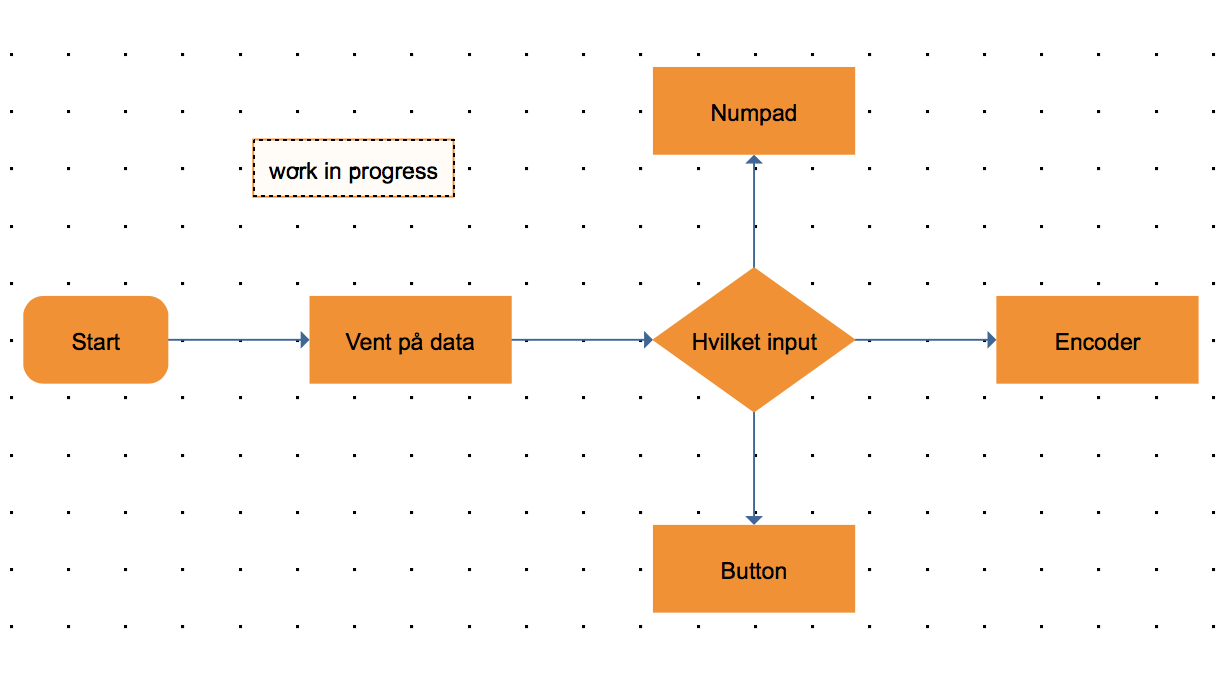
\includegraphics[width=15cm]{billeder/ui_flowchart}
	\caption{Menusystemets opbygning beskrevet med et flowchart. \husk{Søren}{WIP!}}
\end{figure}

Menusystemet sørger for at "lytte" efter eventuelt indkommende data, og skal, når der er data tilgængeligt, behandle den derefter. I denne buffer kan der være tre forskellige ting som har indflydelse på hvad der skal ske. Der er på "EMP-board"'et en numpad, dedikerede knapper, og en encoder. LCD'en er det hovedsagelige i UI'et, da det er her brugeren kan se hvor i menuen man er, samt se hvad indstillingerne er og hvad de eventuelt skal ændres til.

\section{I$^2$C}\label{sec:i2c}
For at implementere et kommunikationssystem til at styre equalizeren, bruges I$^2$C. På den måde kan en anden microcontroller kommunikere og ændre indstillinger og profiler. Da EMP-boardet ikke bruges, og der derfor ikke er noget LCD display, er dette umiddelbart den bedste løsning. På den måde tager vi også en del load af selve EQ-mikrokontrolleren, da User Interfacet foregår på en ekstern mikrokontroller.

Dette gør det også nemmere at senere tilføje moduler til User Interfacet, da I$^2$C protokollen allerede er trådt i kraft, og man kun behøver at ændre kode på den eksterne mikrokontroller.

\section{LCD Display}\label{sec:lcd}
LCD displayet viser equalizerens status informationer. Man kan se den igangværende eq-profil - altså hvilken lydindstilling der aktuelt kører. Derudover er der et VU-meter, som bliver brugt til at se om der er signal igennem, samt hvor højt det er. På den måde kan man se om den overstyrer. Til sidst er der en CPU-load indikator. Med denne indikator kan der afgøres om der er plads til at indsætte endnu et bånd på equalizeren. Problemet med sådan et LCD display, er at det tager for mange CPU-cycles at skrive til, så derfor er der implementeret en metode til at håndtere dette. \\

Da der som tidligere nævnt kun er 1814 CPU-cycles mellem hver interrupt/sample, kan hele LCD'en ikke opdateres på en gang, da dette ville tage mere end 1814 cycles. Derfor er der implementeret en buffer, hvor den skriver til ét felt på LCD'en, ved hver interrupt. Det tager ingen tid at skrive til denne buffer, så derfor spares der på CPU-cycles, så de kan bruges til noget der er vigtigere (f.eks. DSP). Da LCD'en så har sin egen task, kan den skrive bufferen når der er tid til det. 